\documentclass[12pt,english]{article}
\usepackage[a4paper,bindingoffset=0.2in,%
            left=1in,right=1in,top=1in,bottom=1in,%
            footskip=.25in]{geometry}
\usepackage{blindtext}

\usepackage[english]{babel}
\usepackage[utf8]{inputenc}
\usepackage{amsmath}
\usepackage[colorinlistoftodos]{todonotes}
\usepackage{graphicx}

\usepackage[backend=bibtex]{biblatex}
\addbibresource{mybib.bib}
\usepackage[hidelinks]{hyperref}


\title{Correlation between Professional Domain and Facial Features based on Face Clustering}

\author{Bithiah Yuan}

\date{\today}

\begin{document}

\maketitle

%\begin{abstract}
%Bitcoin as an electronic payment system prevents the double-spending problem using the Proof-of-Work confirmation protocol. However, security issues arise with fast payments using Bitcoin as merchants are required to exchange their goods in a short time. We examine double-spending attacks on fast-payments and show how the attacks can be executed. Moreover, we demonstrate how the countermeasures by Bitcoin developers are either ineffective or produce additional costs for the merchants. Ultimately, we present an easy and lightweight solution for the dection of double-spending attacks in fast payments.


%\end{abstract}

\section{Introduction}
\label{sec:introduction}

\quad 
A significant source of information and attributes can be derived from the human face by non-verbal communication \cite{joo}. As a result, facial features have been studied extensively in the social-science domain to predict success in reaching reputable leadership positions. In particular, studies have shown that certain facial features contribute to higher salaries and more prestigious employments for CEOs. In application, the relationship between facial characteristics and social attributes can provide an more powerful objective indicator for organizations to idenity and select effective leaders within their domain than broad facial cues such as attractiveness and competence. Results have shown that a human judge can identify business, military, and sports leaders from their faces with above-chance accuracy. However, these results are biased and do not imply the actual leadership qualities of a person \cite{olivola}.

Caused by behaviour experiments from human judgement, the the research of the social attributes and facial features in the social-sciences are limited in scalability, consistency, and generalization. For example, prior familiarity to the faces of the study and personal preferences can affect the results. Therefore, a growing number of social trait judgment studies have been extended and refined to computer vision and machine learning research due to the capability of using massive datasets and large-scale processing capacity \cite{joo}.

Through a computational framework, \cite{joo} examined the relationship between facial traits and the social construction of leadership by a trained model that can predict the outcomes of political elections based on the perceived social attributes of a person's appearance. The results indicate that similar methods can be used to predict behavior in a broad range of human social relations, such as mate selection, job placement,and political and commercial negotiations \cite{joo}.

Clustering analysis is an unsupervised learning technique that groups data points into clusters based on their similarities. It is useful in grouping a collection of unlabeled data with similar nature into clusters. \cite{shi} investigated clustering a large number of unlabeled face images into individual identities present in the data \cite{shi}. The workflow shown in Figure\ref{fig:face} consists of obtaining face representations of a collection of unlabeled date by a deep neural network. The choice of clustering algorithm then groups the face images according to their identity.

Motivated by the researches in computational social trait judgment and \cite{shi}, the following paper aims to examine the correlation between a person's profession based on their facial features through clustering face images. The clustering problem consists of the face representation and similarity metric of the face images and the choice of clustering algorithm \cite{shi}. Due to the importance of the underlying face representation in face clustering, this paper further compares different open-source state-of-the-art feature extraction methods based on deep learning.\\

\begin{figure}[!tbp]
 \centering
    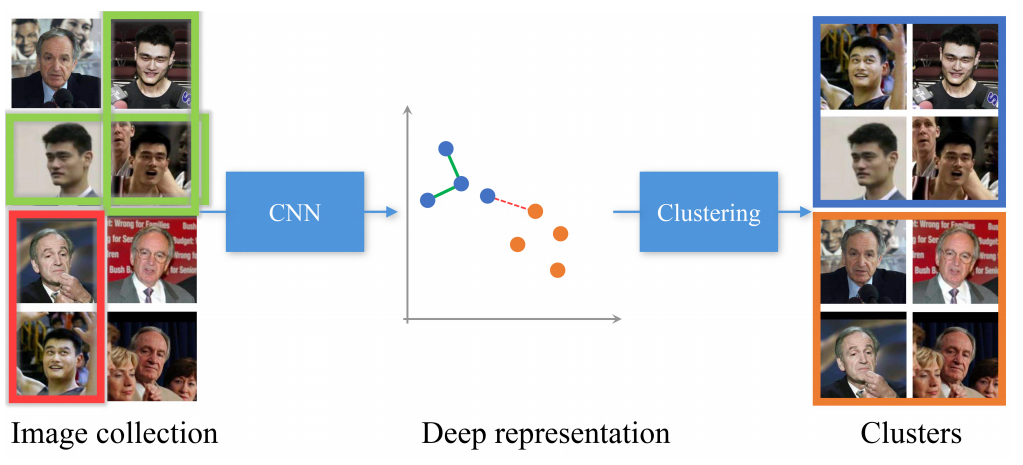
\includegraphics[width=\textwidth]{figures/otto_faceClustering_workflow.png}
    \caption{Face clustering workflow \cite{shi}}
	\label{fig:face}
\end{figure}

\section{Background}	

\subsection{Face Recognition}

\quad
Face recognition focuses on identifying or verifying the identity of subjects in images or videos \cite{trigueros}. Challenges occur in real world (in-the-wild) images due to variations ranging from head poses and illumination conditions to aging and facial expressions. Recently, deep learning methods based on convolutional neural networks (CNNs) were able to achieve very high accuracy by learning robust features due to the availability of large-scale faces in-the-wild datasets on the web \cite{trigueros}. 

Face recognition systems are usually composed of the following 4 steps \cite{trigueros}: 

\begin{enumerate}
  \item Face Detection:\\ Detect the position of the faces in an image and returns the coordinates of a bounding box for each face as shown in Figure \ref{fig:detect}.
  \item Face Alignment: \\ Find a set of facial landmarks with the best affine transformation that fits a set of reference points located at fixed locations in the image as shown in Figure \ref{fig:landmark}.
  \item Face Representation: \\ Trasnform the pixel values of a face image into a discriminative feature vector.
  \item Face Matching: \\ Compute similarity scores from feature vectors.
\end{enumerate} 
 
\begin{figure}[!tbp]
  \centering
  \begin{minipage}[b]{0.49\textwidth}
    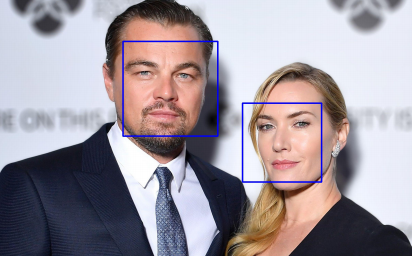
\includegraphics[width=\textwidth]{figures/face_detection.png}
    \caption{Face Detection \cite{trigueros}}
    \label{fig:detect}
  \end{minipage}
  \hfill
  \begin{minipage}[b]{0.49\textwidth}
    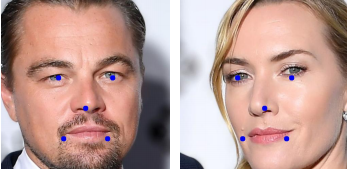
\includegraphics[width=\textwidth]{figures/landmark.png}
    \caption{Face Alignment \cite{trigueros}}
    \label{fig:landmark}
  \end{minipage}
\end{figure}



\subsection{Feature Extraction}

\subsection{Clustering}
  

\section{Experiment}

\subsection{Dataset}


\subsection{Evaluation}


\section{Conclusion}

\nocite{*}

\printbibliography

\end{document}